\chapter{Inequalities}
Till now we were dealing with the cases where $f(x)=g(y)$. The thing to note is that they were mostly equal. This is normally not true in real life. Say you have a budget of $10,000$ dollars for your wedding. Our expenditure needs to be less than or equal to $10,000$ dollars. I don't thing people will hold it against you for saving money.\\
This chapter doesn't use $=$ much. Instead we'll have two sides which will not be equal.\\
\section{Another note on notation}
We will make use of two new notations, $\sum_{\text{cyc}}$ and $\sum_{\text{sym}}$ which mean to cycle through all the $n$ values and go through all the $n!$ values respectively. For example:\\
$\sum_{\text{cyc}}a^2=a^2+b^2+c^2+d^2\\
\sum_{\text{cyc}}ab=ab+bc+ca+ad\\
\sum_{\text{sym}}a^2=6(a^2+b^2+c^2+d^2)\\
\sum_{\text{sym}}ab=ab+ac+ad+bc+bd+ad\\$
\section{AM-GM and Muirhead}
\begin{theorem}
[AM-GM]
    \[\frac{x_1 + x_2 + \ldots + x_n}{n} \geq \sqrt[n]{x_1 \cdot x_2 \cdot \ldots \cdot x_n}\]
    The equality holds, if and only if, $x_1=x_2=x_3\dots=x_n$
\end{theorem}
\begin{proof}
    AM-GM can be proven in various ways. However, the simplest and most logical one is presented here.\\
    We'll refer to the inequality as $I_n$ with $n$ being the number of terms. \\
    Let's first prove it for $n=2$.\\
    Let $x_1+k=x_2$. Proof by induction:\\
    (B) for $k=1$, $(\frac{x_1+x_1+1}{2})^2\\
    =(x_1+\frac{1}{2})^2\\
    =x_1^2+x_1+\frac{1}{4}
    > x_1(x_1+1)=x_1^2+x_1$\\
    (S) Let's assume this is true for some $k$ leading to $x_1^2+kx_1+\frac{k^2}{4}>x_1(x_1+k)$, then:\\
    $x_1(x_1+k+1)\\
= x_1^2+kx_1+x_1\\
= x_1(x_1+k)+x_1\\
< x_1^2+kx_1+\frac{k}{4}+x_1\\
< x_1^2+(k+1)x_1+\frac{(k+1)^2}{4}$\\
Hence, proved.\\
Now with this information,  let's do something unique. Assuming, $I_n$ holds, let's prove that $I_{2n}$ also holds.\\
Let $x_1, x_2, \ldots, x_{2n}$ be any list of nonnegative reals. Then, because the two lists $x_1, x_2 \ldots, x_n$ and $x_{n+1}, x_{n+2}, \ldots, x_{2n}$, each have $n$ variables,
\[\frac{x_1 + x_2 + \cdots + x_n}{n} \geq \sqrt[n]{x_1 x_2 \cdots x_n}\] and\\
\[\frac{x_{n+1} + x_{n+2} + \cdots + x_{2n}}{n} \geq \sqrt[n]{x_{n+1} x_{n+2} \cdots x_{2n}}.\]
Adding these two inequalities together and dividing by $2$ yields\[\frac{x_1 + x_2 + \cdots + x_{2n}}{2n} \geq \frac{\sqrt[n]{x_1 x_2 \cdots x_n} + \sqrt[n]{x_{n+1} x_{n+2} \cdots x_{2n}}}{2}.\]
Using $I_2$, on $\sqrt[n]{x_1 x_2 \cdots x_n}$ and $\sqrt[n]{x_{n+1} x_{n+2} \cdots x_{2n}}$ we get
\[\frac{\sqrt[n]{x_1 x_2 \cdots x_n} + \sqrt[n]{x_{n+1} x_{n+2} \cdots x_{2n}}}{2} \geq \sqrt[2n]{x_1 x_2 \ldots x_{2n}}.\]\\Plugging this in proves this for $I_{2n}$\\
Finally, we'll perform the third and final (S) this time we'll assume that $I_n$ holds and prove that so does $I_{n-1}$, causing all the dominos to topple.\\
Letting $x_n = \frac{x_1 + x_2 + \cdots + x_{n-1}}{n-1}$, we have that\[\frac{x_1 + x_2 + \cdots + x_{n-1} + \frac{x_1 + x_2 + \cdots + x_{n-1}}{n-1}}{n} \geq \sqrt[n]{x_1 x_2 \cdots x_{n-1} \left(\frac{x_1 + x_2 + \cdots + x_{n-1}}{n-1}\right)}.\]Because we assumed AM-GM in $n$ variables, equality holds if and only if $x_1 = x_2 = \cdots = x_{n-1} = \frac{x_1 + x_2 + \cdots + x_{n-1}}{n-1}$. However, note that the last equality is implied if all the numbers of $x_1, x_2, \ldots, x_{n-1}$ are the same; thus, equality holds if and only if $x_1 = x_2 = \cdots = x_{n-1}$.

We first simplify the lefthand side. Multiplying both sides of the fraction by $n-1$ and combining like terms, we get that\[\frac{x_1 + x_2 + \cdots + x_{n-1} + \frac{x_1 + x_2 + \cdots + x_{n-1}}{n-1}}{n} = \frac{nx_1 + nx_2 + \cdots + nx_{n-1}}{n(n-1)} = \frac{x_1 + x_2 + \cdots + x_{n-1}}{n-1}.\]Plugging this into the earlier inequality yields\[\frac{x_1 + x_2 + \cdots + x_{n-1}}{n-1} \geq \sqrt[n]{x_1 x_2 \cdots x_{n-1} \left(\frac{x_1 + x_2 + \cdots + x_{n-1}}{n-1} \right)}.\]Raising both sides to the $n$th power yields\[\left( \frac{x_1 + x_2 + \cdots + x_{n-1}}{n-1}\right)^n \geq x_1 x_2 \cdots x_{n-1}\left(\frac{x_1 + x_2 + \cdots + x_{n-1}}{n-1}\right).\]From here, we divide by $\frac{x_1 + x_2 + \cdots + x_{n-1}}{n-1}$ and take the $(n-1)^{\textrm{th}}$ root to get that\[\frac{x_1 + x_2 + \cdots + x_{n-1}}{n-1} \geq \sqrt[n-1]{x_1 x_2 \cdots x_{n-1}}.\]This is $I_{n-1}$. \\
With the most advanced thing we have used and will probably use in induction, we can finally say:\\
Hence, proved.\\
\end{proof}
This theorem is the king of inequalities. A lot of people believe it to be one of the most important facts in maths. It stands for 'arithmetic mean, geometric mean'. While it is quite a well known inequality, it's proof is less known. If you ever find yourself having crush on a math lover, just present this proof from memory. Thank me later.\\
Now back to math, We can use AM-GM to get the following things:\\
$a^2+b^2 \geq 2ab$ and $a^3+b^3+c^3 \geq 3abc$\\
You can sum such inequalities to solve simple questions.\\
\begin{example}
    For $a, b, c > 0$ prove that $a^2+b^2+c^2 \geq ab + bc + ca$
\end{example}
\begin{proof}
    As we just discussed above, $a^2+b^2 \geq 2ab$, $b^2+c^2 \geq 2bc$, $c^2+a^2 \geq 2ac$. Adding them gives us:\\
    $2a^2+2b^2+2c^2 \geq 2ab+2bc+2ca\\
    \therefore a^2+b^2+c^2 \geq ab+bc+ca$\\
\end{proof}
\begin{example}
    For $a, b, c > 0$ prove that $a^4+b^4+c^4 \geq a^2bc+ab^2c+abc^2$
\end{example}
\begin{proof}
    $a^4+a^4+b^4+c^4 \geq 4a^2bc$\\
    $a^4+b^4+b^4+c^4 \geq 4ab^2c$\\
    $a^4+b^4+c^4+c^4 \geq 4abc^2$\\
    Adding these gives us the inequality.
\end{proof}
In most symmetric inequality, both sides will be equal when
we set all variables equal.\\
Moreover, we often compare expressions which are the same degree, or homogeneous. For example when we write $a^2 + b^2 + c^2 \geq ab + bc + ca$, both sides are degree 2. (Notice that the AM-GM inequality itself has the same property!) \\
The reason for this is $x^5$ and $x^3$ are not comparable for generic $x > 0$, since the behaviors when $x$ is very small and x is very large are different. So a non-homogeneous inequality like $a^2+b^2+c^2 \geq a^3+b^3+c^3$ will definitely not be true in general, since the behaviors if $a=b=c=0.01$ and $a=b=c=100$ will be different. You may have already picked up some intuition: more “mixed” terms are smaller. For example, for degree 3, the polynomial $a^3 +b^3 +c^3$ is biggest and $3abc$ is the smallest. Roughly, the more “mixed” polynomials are the smaller.\\
This intuition can be formalized as Muirhead inequality\\
\begin{definition}
     If $x_1+x_2+\dots + x_k \geq y_1 + y_2+ \dots + y_k$ for all $0\leq k \leq n$ then ${x_1,x_2,\dots,x_n} \succ {y_1,y_2,\dots,y_n}$
\end{definition}
The $\succ$ symbol in speaking changes to majorizes. Using this definaion, we can say
   \begin{theorem}
   [Muirhead]
    \[\sum_{\text{sym}}a_1^{x_1}a_2^{x_2}\dots a_n^{x_n} \geq \sum_{\text{sym}}a_1^{y_1}a_2^{y_2}\dots a_n^{y_n}\]
    If $x_1,x_2,x_3 \dots x_n \succ y_1,y_2,y_3 \dots y_n$
\end{theorem}
Since, $(5,0,0)\succ(3,1,1)\succ(2,2,1)$\\
$a^5+a^5+b^5+b^5+c^5+c^5 \geq a^3bc+a^3bc+ab^3c+ab^3c+abc^3+abc^3 \geq a^2b^2c+a^2b^2+ab^2c^2+ab^2c^2+a^2bc^2+a^2bc^2$\\
Note: It is symmetric, not cyclic. Our only tool for cyclic is still AM-GM.\\
\section{Non-homogeneous equations}
\subsection{Even's Substitution}
If an inequality has the condition $abc = 1$, one can also sometimes use the substitution $(a, b, c) = (x/y, y/z, z/x)$ which will transform it into a homogeneous inequality automatically. I call it the Even's substitution as I first learnt it from Evan Chan's handouts(Its not an official name.).
\begin{example}
    Prove that if $abc = 1$ then $a^2 + b^2 + c^2 \geq a + b + c$
\end{example}
\begin{proof}
    Using Evan's substitution, the problem statement transforms to
    $\frac{x^2y^4+y^2z^4+z^2x^4}{x^2y^2z^2}\geq \frac{xy^2+yz^2+zx^2}{xyz}\\
    \iff x^2y^4+y^2z^4+z^2x^4 \geq x^2y^3z + xy^2z^3 + x^3yz^2$\\
    Using, $4x^2y^4+y^2z^4+z^2x^4 \geq 6x^2y^3z$, and adding its cycles, we get the inequality.
\end{proof}
\subsection{Ravi's Substitution}
Sometimes, an inequality will refer to the $a, b, c$ as the sides of a triangle. In that case, one can replace $(a, b, c) = (y + z, z + x, x + y)$ where $x, y, z > 0$ are real numbers using the properties of in-circle. \\
\begin{figure} [h]
    \centering
    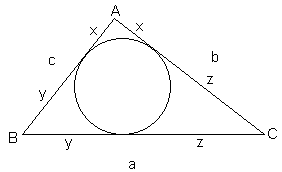
\includegraphics[width=0.5\linewidth]{Photos/Ravi's substitution.png}
    \caption{Ravi's Substitution}
    
\end{figure}
This is colloquially known as the Ravi substitution, after Ravi Vakil, a well known math professor at Stanford and an IMO gold medalist(and 4 time Putnam fellow)
\begin{example}
     Find the smallest constant k such that
$k>\frac{a^2+b^2+c^2}{ab+bc+ca}$
where $a,b,c$ are the sides of a triangle.
\end{example}
\begin{proof}
    Using Ravi's Substitution,\\
    $\frac{a^2+b^2+c^2}{ab+bc+ca}\\
    =\frac{(x+y)^2+(y+z)^2+(z+x)^2}{(x+y)(y+z)+(y+z)(z+x)+(x+z)(x+y)}\\
    =\frac{2(x^2+y^2+z^2+xy+yz+xz)}{x^2+y^2+z^2+3(xy+yz+zx)}$\\
    Hence we are looking for k such that:\\
    $k(x^2+y^2+z^2)+3k(xy+yz+zx)> 2(x^2+y^2+z^2)+2(xy+yz+xz)\\
    (3k-2)(xy+yz+zx)>(2-k)(x^2+y^2+z^2)$\\
    We already know that $x^2+y^2+z^2 > xy+yz+zx$; Hence,\\
    $(3k-2)(x^2+y^2+z^2)>(2-k)(x^2+y^2+z^2)\\
    3k-2 > 2-k\\
    4k > 4\\
    k > 1$\\
    Thus, minimum value of k is 1.
\end{proof}
\subsection{Schur's Inequality}
It's canny how the three tools for non homogeneity all are named after someone but for completely different reasons. This one was discovered by Issai Schur, the Russian mathematician and is hence named after him.
\begin{theorem}
[Schur's Inequality]
     For all non-negative $a,b,c \in \mathbb{R}$ and $r>0$:
\[a^r(a-b)(a-c)+b^r(b-a)(b-c)+c^r(c-a)(c-b) \geq 0\]
The four equality cases occur when $a=b=c$ or when two of $a,b,c$ are equal and the third is ${0}$.
\end{theorem}
\begin{proof}
    Let $a\geq b\geq c$.\\
    $\therefore a^r(a-b)(a-c)+b^r(b-a)(b-c)\\
    = a^r(a-b)(a-c)-b^r(a-b)(b-c)\\
    = (a-b)(a^r(a-c)-b^r(b-c))$\\ 
    Clearly, $a^r \geq b^r \geq 0$, and $a-c \geq b-c \geq 0$.\\ 
    Thus, $(a-b)(a^r(a-c)-b^r(b-c)) \geq 0\\
    \therefore a^r(a-b)(a-c)+b^r(b-a)(b-c) \geq 0$.\\ 
    As, $c^r(c-a)(c-b) \geq 0\\
    \therefore a^r(a-b)(a-c)+b^r(b-a)(b-c)+c^r(c-a)(c-b) \geq 0$.
\end{proof}

\section{Some advanced inequalities}
\subsection{Extended AM-GM}
\begin{theorem}
    [Weighted Power Mean] For $a_1,a_2,a_3 \dots a_n$ positive reals and $w_1,w_2, w_3, \dots w_n$ where $w_1+w_2+w_3+\dots +w_n=1$. For any real number R, we'll define the weighted power mean as:\\
   \[P(x)=\begin{cases}
       (w_1a_1^r+w_2a_2^r \dots +w_na_n^r)^{1/r} & r \neq 0\\
       a_1^{w_1}a_2^{w_2} \dots a_n^{w_n} & r=0\\
   \end{cases}\]
   Then, if $k>l$ then $P(k) \geq P(l)$. Equality occurs when $a_1=a_2=\dots=a_n$\\
    \end{theorem}
\begin{theorem}
    [Simplified Weighted Mean] The $r^{th}$ power mean refers to:\\
    \[p(x)=\begin{cases}
       (\frac{a_1^r+a_2^r \dots +a_n^r}{n})^{1/r} & r \neq 0\\
       \sqrt[n]{a_1a_2\dots a_n} & r=0\\
   \end{cases}\]\\
   Basically, we have set $w_1=w_2=\dots=w_n=\frac{1}{n}$. The inequality still holds true, if $k>l$ then $P(k) \geq P(l)$. Equality occurs when $a_1=a_2=\dots=a_n$
\end{theorem}
Using the Simplified Weighted Mean, and setting $r$ to $(2,1,0,-1)$ respectively will give us:\\
\begin{theorem}[RMS-AM-GM-HM]
    \begin{align*}
\sqrt{\frac{a_1^2 + a_2^2 + \ldots + a_n^2}{n}} &\geq \frac{a_1 + a_2 + \ldots + a_n}{n} \\
&\geq \sqrt[n]{a_1 \cdot a_2 \cdot \ldots \cdot a_n} \\
&\geq \frac{n}{\frac{1}{a_1} + \frac{1}{a_2} + \ldots + \frac{1}{a_n}}
\end{align*}
\end{theorem}
I'll not prove any of these. While RMS-AM-GM-HM can be proven using the same mechanism we used to prove AM-GM, the weighted form will use some math which we are yet to explore. That technique appears in chapter 15\\
\subsection{Cauchy-Schwarz(aka SEBACS)}
The following theorem is taught under many names. Cauchy had originally proposed it, it was generalized by Schwarz and Bunyakovsky, given an Olympiad friendly form by Arthur Engel and popularized by Titu Andreescu and Nairi Sedrakyan.  I propose it being called SEBACS Inequality.
\begin{theorem}
    [Orignal Form]
    for any list of reals $a_1, a_2, \ldots, a_n$ and $b_1, b_2, \ldots, b_n$,\[(a_1^2 + a_2^2 + \cdots + a_n^2)(b_1^2 + b_2^2 + \cdots + b_n^2) \geq (a_1b_1 + a_2b_2 + \cdots + a_nb_n)^2,\]\\
\end{theorem}
\begin{theorem}
[Mordern Form]
for any list of reals $a_1, a_2, \ldots, a_n$ and $b_1, b_2, \ldots, b_n$:\\
\[\frac{ a_1^2 } { b_1 } + \frac{ a_2 ^2 } { b_2 } + \cdots + \frac{ a_n ^2 } { b_n } \geq \frac{ (a_1 + a_2 + \cdots+ a_n ) ^2 } { b_1 + b_2 + \cdots+ b_n }.\] 
\end{theorem}
Proving any of these will require us to use vectors which we'll learn later(in geometry). With them it will become quite trivial and we'll prove it then. The non-geometrical proof is found in chapter 15\\
For now, let's try an example:
\begin{example}
    for positive $a, b, c$, prove that
$\frac{a}{b+c} + \frac{b}{c+a} + \frac{c}{a+b} \ge \frac{3}{2}$,
\end{example}
\begin{proof}
    By SEBACS Inequality:\\
    $[\sqrt{(b+c)}^2 + \sqrt{(c+a)}^2 + \sqrt(a+b)^2]\left( \sqrt{\frac{1}{b+c}}^2 + \sqrt{\frac{1}{c+a}}^2 + \sqrt{\frac{1}{a+b}}^2 \right) \geq (\sqrt{\frac{b+c}{b+c}}+\sqrt{\frac{a+c}{a+c}}+\sqrt{\frac{b+a}{b+a}})^2$,\\
    Upon expanding this gives us:\\
    $2\left( \frac{a+b+c}{b+c} + \frac{a+b+c}{c+a} + \frac{a+b+c}{a+b} \right) \geq 9\\
   \iff \frac{a}{b+c} + \frac{b}{c+a} + \frac{c}{a+b} \ge \frac{3}{2}$
\end{proof}
\section{A note}
A lot of more advanced inequalities need calculus for complete exploration. Hence, we've decided to explore them in greater detail in Chapter-15.  Inequalities tend to not occur in lower levels and occur at an advanced state at higher level. Hence, we have been unable to include a lot of PYQs here. 
\begin{xcb}{Exercises}
\begin{enumerate}
\item Prove that $a^5 + b^5 + c^5 \geq a^3bc + b^3ca + c^3ab \geq abc(ab + bc + ca).$
\item (PRMO) What is the largest positive integer n such that $\frac{a^2}{\frac{b}{29} +\frac{c}{31}} +\frac{b^2}{\frac{c}{29}+\frac{a}{31}} +\frac{c^2}{\frac{a}{29}+\frac{b}{31}}\geq n(a+b+c)$
\item For a,b,c the sides of some triangle, prove the inequality $\dfrac{1}{b+c-a}+\dfrac{1}{c+a-b}+\dfrac{1}{a+b-c}\ge\dfrac1a+\dfrac1b+\dfrac1c$ 
\item (Candian MO) For positive reals $a,b,c$, \\
\[\frac{a^3}{bc}+\frac{b^3}{ac}+\frac{c^3}{ab} \geq a+b+c\]
\item Prove that for any non-negative $a,b,c$:\\
\[\frac{a}{b+c}+\frac{b}{a+c}+\frac{c}{a+b}\geq \frac{3}{2}\]
\item Prove that:\\
$\sqrt{a_1^2+a_2^2+\dots}+\sqrt{b_1^2+b_2^2+\dots} \geq \sqrt{(a_1+b_1)^2+(a_2+b_2)^2+\dots}$
\item If $a,b,c>0$, prove that:\\
\[a^3b+b^3c+c^3a \geq abc(a+b+c)\]\\
\item (IMO 1995) Let $a, b, c$ be positive real numbers such that $abc = 1$. Prove that\[\frac{1}{a^3(b+c)} + \frac{1}{b^3(c+a)} + \frac{1}{c^3(a+b)} \geq \frac{3}{2}.\]
\item If $\frac{1}{a}+\frac{1}{b}+\frac{1}{c}=1$, then $(a + 1)(b + 1)(c + 1) \geq 64$\\
\item . If $abcd = 1$, then $a^4b + b^4c + c^4d + d^4a \geq a + b + c + d$.
\item Prove that:\\
$\frac{a}{b+c}+\frac{b}{a+c}+\frac{c}{a+b} \geq  \frac{3}{2}$\\
for any non-negative $a, b, c$\\
\item If $a, b, c > 0$ prove that\\
$abc(a + b + c) \geq a^3b + b^3c + c^3a$\\
\item For $a,b,c > 0$, prove that:\\
$abc \geq (a + b - c)(b + c - a)(c + a - b)$
\item Let $a, b, c, d$ be non-negative real numbers such that $a + b + c + d = 1$. Find the minimum value of $a^2 + b^2 + c^2 + d^2$\\
\item (AMC 10) Let $A$, $M$, and $C$ be nonnegative integers such that $A+M+C=10$. What is the maximum value of $A\cdot M\cdot C+A\cdot M+M\cdot C+C\cdot A$?
\item (AMC 10) Let $a,b,$ and $c$ be real numbers such that
\[a+b+c=2, \text{ and}\]\[a^2+b^2+c^2=12\]
What is the difference between the maximum and minimum possible values of $c$?
\item  (MPFG) Find the least real number K such that for all real numbers $x$ and $y$, we have
$(1 + 20x^2)(1 + 19y^2)\geq Kxy$
\item Prove that \[\frac{x}{x+y}+\frac{y}{y+z}+\frac{z}{z+x} \leq 2\]
\end{enumerate}
\end{xcb}